\chapter{Introduction}\label{ch:intro}
\section{Motivation and Background}
\subsection{Emergence of Networked Autonomous Systems}
Over the past two decades, multi-agent systems (MAS) have transitioned from theoretical abstractions to critical infrastructure across modern engineering domains. AI, especially agentic AI, Distributed vehicular platoons, unmanned aerial vehicle (UAV) swarms, robotic cooperative manipulation teams, and decentralized smart microgrids, all rely on distributed coordination algorithms. Compared to traditional centralized control architectures, distributed frameworks offer significant advantages:
\begin{itemize}
    \item \textbf{Scalability:} Computational load is distributed across individual agent nodes, avoiding exponential growth in processing overhead at a central server. 
    \item \textbf{Spatial Coverage and Flexibility:} Localized interaction topologies enable large - scale geographic deployment, allowing swarms to adapt to changing environments dynamically.
    \item \textbf{Fault Tolerance:} Eliminating single points of failure ensures that the loss or degradation of an individual node does not compromise the global mission.
\end{itemize}
A fundamental requirement in all multi-agent coordination problems is achieving consensus-- a state where a group of autonomous agents reaches agreement on a shared physical or virtual variable (such as position, velocity, heading, or phase) relying solely on local inter-agent communication.

\subsection{Topologies, Information Flow, and Graph Theory Fundamentals}
In networked multi-agent systems, the interaction structure among agents is modelled using graph theory \cite{godsil2001algebraic, mesbahi2010graph}. Let $\G = (\Vg, \Eg, \Wg)$ represent a weighted directed graph (digraph).
\begin{definition}[Weighted Directed Graph \cite{mesbahi2010graph, ren2008consensus}]\label{def:weighted_digraph}
A weighted directed graph (or digraph) is defined as a triplet $\G = (\Vg, \Eg, \Wg)$, where:
\begin{enumerate}
    \item $\Vg = \{1, 2, \dots, N\}$ is a finite, non-empty set of $N$ discrete nodes or vertices, with $N = |\Vg|$ representing the total number of autonomous agents in the network.
    \item $\Eg \subseteq \Vg \times \Vg$ is the set of directed edges (or arcs) representing directed information channels. An ordered pair $(j, i) \in \Eg$ denotes a directed edge originating at tail node $j$ and terminating at head node $i$. In this setup, information flows strictly from agent $j$ to agent $i$; node $j$ is classified as a parent/neighbor of node $i$, and node $i$ is classified as a child of node $j$. Self-loops are excluded, i.e., $(i, i) \notin \Eg, \forall i \in \Vg$.
    \item $\Wg = [w_{ij}] \in \R^{N \times N}$ is the weighted adjacency matrix. The matrix entry $w_{ij}$ represents the non-negative weight associated with the edge $(j, i) \in \Eg$:
    \begin{equation}\label{eq:adj_matrix_def}
        w_{ij} = \begin{cases}
            > 0, & \text{if } (j, i) \in \Eg \\
            0, & \text{otherwise}
        \end{cases}
    \end{equation}
    For an unweighted graph, $w_{ij} = 1$ whenever $(j, i) \in \Eg$.
\end{enumerate}
\end{definition}

\begin{definition}[Neighbor Sets and In-Degree Matrix \cite{ren2008consensus, mesbahi2010graph}]\label{def:neighbor_set}
The set of in - neighbors of agent $i$, denoted by $\mathcal{N}_i$, consists of all nodes from which agent $i$ receives direct state information:
\begin{equation}
    \mathcal{N}_i = \{j \in \Vg : (j, i) \in \Eg\}
\end{equation}
The weighted in-degree of node $i$, denoted by $d_{\text{in}, i}$, is the sum of the weights of all incoming edges to node $i$:
\begin{equation}
    d_{\text{in}, i} = \sum_{j \in \mathcal{N}_i} w_{ij} = \sum_{j=1}^{N} w_{ij}
\end{equation}
The network in-degree matrix $\Dg \in \R^{N \times N}$ is a diagonal matrix containing the in-degrees of all agents:
\begin{equation}\label{eq:indegree_matrix}
    \Dg = \text{diag}(d_{\text{in}, 1}, d_{\text{in}, 2}, \dots, d_{\text{in}, N})
\end{equation}
\end{definition}

\begin{definition}[Node Graph Laplacian Matrix \cite{godsil2001algebraic, mesbahi2010graph}]\label{def:ch_intro_graphLaplacian}
The node graph Laplacian matrix $\mathcal{L} \in \R^{N \times N}$ associated with the graph $\G$ is defined as:
\begin{equation}\label{eq:laplacian_def}
    \mathcal{L} = \Dg - \Wg
\end{equation}
where $\Dg = \text{diag}(d_{in,1}, d_{in,2}, \dots, d_{in,N})$ is the in-degree matrix with diagonal elements $d_{in,i} = \sum_{j=1}^{N} w_{ij}$.\\
Element-wise, the elements of the Laplacian matrix $[\mathcal{L}]_{ij} \eqqcolon l_{ij}$ are given by:
\begin{equation}\label{eq:ch_intro_laplacianentries}
    l_{ij} = \begin{cases}
        \sum_{k=1, k \neq i}^{N} w_{ik}, & \text{if } i = j \\
        -w_{ij}, & \text{if } i \neq j
    \end{cases}
\end{equation}
\end{definition}
\begin{remark}[Spectral Properties of the Laplacian \cite{ren2005second, mesbahi2010graph}]\label{prop:ch_intro_laplacianzeroeig}
\leavevmode\par\noindent
The graph Laplacian $\mathcal{L}$ exhibits the following fundamental spectral properties:
\begin{enumerate}
    \item \textbf{Row-Sum Property and Zero Eigenvalue:} By definition \eqref{eq:ch_intro_laplacianentries}, the sum of entries along every row of $\mathcal{L}$ is identically zero:
    \begin{equation}
        \sum_{j=1}^{N} l_{ij} = d_{\text{in}, i} - \sum_{j=1, j \neq i}^{N} w_{ij} = 0, \quad \forall i \in \{1, 2, \dots, N\}
    \end{equation}
    This establishes that $\mathcal{L} \mathbf{1}_N = 0_{N \times 1}$, where $\mathbf{1}_N = [1, 1, \dots, 1]^T \in \R^N$ is the vector of all ones. Thus, $\lambda_1 = 0$ is always an eigenvalue of $\mathcal{L}$ with a corresponding right eigenvector $\mathbf{1}_N$.
    
    \item \textbf{Positive Real Spectrum Location:} By Gershgorin's Disc Theorem, all eigenvalues $\lambda \in \sigma(\mathcal{L})$ lie within the union of closed discs centered at $l_{ii} = d_{\text{in},i}$ with radii $R_i = \sum_{j \neq i} |l_{ij}| = d_{\text{in},i}$. Consequently, every eigenvalue satisfies:
    \begin{equation}
        \mathfrak{Re}(\lambda_i) \ge 0, \quad \forall i \in \{1, 2, \dots, N\}
    \end{equation}
    
    \item \textbf{Strict Positivity of Non-Zero Eigenvalues:} If the directed graph $\G$ contains a \emph{directed spanning tree}, then $\lambda_1 = 0$ is a simple eigenvalue (algebraic multiplicity of one), and all remaining $N-1$ non-zero eigenvalues satisfy:
    \begin{equation}
        \mathfrak{Re}(\lambda_i) > 0, \quad \forall i \in \{2, 3, \dots, N\}
    \end{equation}
    ordered by real parts such that $0 = \lambda_1 < \mathfrak{Re}(\lambda_2) \le \dots \le \mathfrak{Re}(\lambda_N)$.
\end{enumerate}
\end{remark}
\subsubsection{Topological Connectivity and Graph Classifications (Directed Graphs)}
The stability and performance of multi-agent protocols depend directly on the structural connectivity of the underlying graph. 
\begin{definition}[Path, Cycle, and Connectivity \cite{godsil2001algebraic}]\label{def:paths_cycles}
\leavevmode\par\noindent
\begin{enumerate}
    \item A \emph{directed path} from node $i_0$ to node $i_k$ is a finite sequence of distinct nodes $(i_0, i_1, \dots, i_k)$ such that $(i_{m-1}, i_m) \in \Eg$ for all $m \in \{1, 2, \dots, k\}$.
    \item A \emph{directed cycle} (or loop) is a directed path that begins and ends at the same vertex, i.e., $i_0 = i_k$, with all intermediate nodes being distinct.
    \item A graph $\G$ is \emph{strongly connected} if there exists a directed path between every pair of distinct vertices $i, j \in \Vg$.
    \item A graph $\G$ contains a \emph{directed spanning tree} if there exists at least one node $r \in \Vg$ (termed the root or leader node) such that a directed path exists from $r$ to every other node $i \in \Vg \setminus \{r\}$. The root node has an in-degree of zero ($d_{\text{in}, r} = 0$) in an acyclic network.
\end{enumerate}
\end{definition}

\begin{definition}[Topological Ordering and Reverse Edges \cite{hao2019role} \cite{dubey2022consensus}]\label{def:topological_ordering}
A graph $\G$ admits a \emph{topological ordering} if its vertices can be indexed as $\{1, 2, \dots, N \}$ such that every directed edge $(j, i) \in \Eg$ satisfies $j < i$.
\begin{enumerate}
    \item Topological ordering is possible if and only if the directed graph $\G$ is acyclic (a Directed Acyclic Graph, or DAG).
    \item Under a topological ordering, the weighted adjacency matrix $\Wg$ and graph Laplacian $\mathcal{L}$ are strictly lower triangular.
    \item A \emph{reverse edge} is a directed edge $(y, x) \in \Eg$ that violates the topological ordering condition, i.e., $y > x$. Adding a reverse edge to an acyclic chain network creates a directed cycle.
    \item The \emph{cycle length} $\ell$ created by a reverse edge from tail node $y$ to head node $x$ is defined as:
    \begin{equation}\label{eq:cycle_length_def}
        \ell = y - x
    \end{equation}
    \begin{remark}
        Note that $\ell$ is defined as one less than the number of nodes participating in the cycle.
    \end{remark}
\end{enumerate}
\end{definition}
\subsubsection{Some Illustrative Numerical Examples}
To illustrate some of these concepts, consider two distinct 5-agent topologies ($N = 5$) with unit edge weights.
\begin{example}[Acyclic Directed Chain with Topological Ordering]\label{example:acyclic_chain_ex}
Consider a 5 agents directed chain as in Figure \ref{fig:acyclic_chain_ex}, where, information flows strictly downstream from Node 1 to Node 5.

\begin{figure}[ht!]
    \centering
    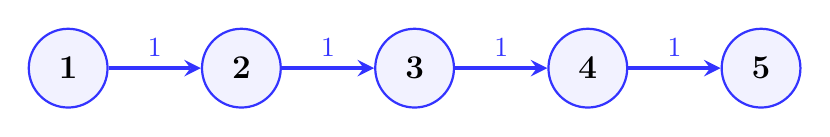
\begin{tikzpicture}[node distance=2.2cm, state/.style={circle, draw=blue!80, fill=blue!5, thick, minimum size=1.0cm, font=\large\bfseries}]
        \node[state] (1) {1};
        \node[state] (2) [right of=1] {2};
        \node[state] (3) [right of=2] {3};
        \node[state] (4) [right of=3] {4};
        \node[state] (5) [right of=4] {5};
        
        \path [->, >=stealth, ultra thick, blue!80] (1) edge node[above] {$1$} (2);
        \path [->, >=stealth, ultra thick, blue!80] (2) edge node[above] {$1$} (3);
        \path [->, >=stealth, ultra thick, blue!80] (3) edge node[above] {$1$} (4);
        \path [->, >=stealth, ultra thick, blue!80] (4) edge node[above] {$1$} (5);
    \end{tikzpicture}
    \caption{A 5-agent directed chain topology with topological ordering.}
    \label{fig:acyclic_chain_ex}
\end{figure}

The adjacency matrix $\mathcal{W}_{\mathcal{G}1}$, in-degree matrix $\mathcal{D}_{\mathcal{G}1}$, and Laplacian matrix $\mathcal{L}_{\mathcal{G}1}$ for this topology are:
\begin{equation*}
\mathcal{W}_{\mathcal{G}1} = \begin{bmatrix} 
0 & 0 & 0 & 0 & 0 \\ 
1 & 0 & 0 & 0 & 0 \\ 
0 & 1 & 0 & 0 & 0 \\ 
0 & 0 & 1 & 0 & 0 \\ 
0 & 0 & 0 & 1 & 0 
\end{bmatrix}, \quad
\mathcal{D}_{\mathcal{G}1} = \text{diag}(0, 1, 1, 1, 1), \quad
\mathcal{L}_{\mathcal{G}1} = \begin{bmatrix} 
0 & 0 & 0 & 0 & 0 \\ 
-1 & 1 & 0 & 0 & 0 \\ 
0 & -1 & 1 & 0 & 0 \\ 
0 & 0 & -1 & 1 & 0 \\ 
0 & 0 & 0 & -1 & 1 
\end{bmatrix}
\end{equation*}
Since $\mathcal{L}_{\mathcal{G}1}$ is strictly lower triangular, its eigenvalues are $\sigma(\mathcal{L}_{\mathcal{G}1}) = \{0, 1, 1, 1, 1\}$. The spectrum is entirely real, with a simple eigenvalue at zero corresponding to the root node (Node 1).
\end{example}

\begin{example}[Directed Chain with a Reverse Edge Forming a Cycle]\label{example:cyclic_chain_ex}
\leavevmode\par \noindent
Now consider the graph shown in Figure \ref{fig:cyclic_chain_ex}, formed by adding a reverse edge from Node 4 to Node 2 ($y = 4, x = 2$) to the chain in Example \ref{example:acyclic_chain_ex}. This creates a directed cycle of length $\ell = 4 - 2 = 2$ involving nodes $\{2, 3, 4\}$.

\begin{figure}[ht!]
    \centering
    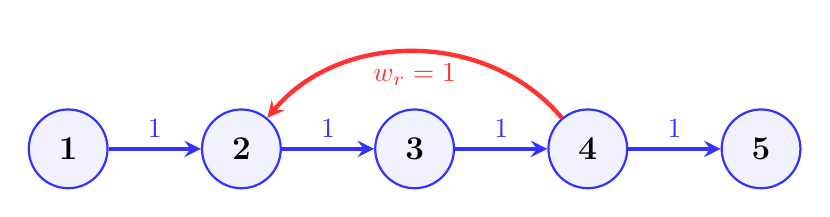
\begin{tikzpicture}[node distance=2.2cm, state/.style={circle, draw=blue!80, fill=blue!5, thick, minimum size=1.0cm, font=\large\bfseries}]
        \node[state] (1) {1};
        \node[state] (2) [right of=1] {2};
        \node[state] (3) [right of=2] {3};
        \node[state] (4) [right of=3] {4};
        \node[state] (5) [right of=4] {5};
        
        \path [->, >=stealth, ultra thick, blue!80] (1) edge node[above] {$1$} (2);
        \path [->, >=stealth, ultra thick, blue!80] (2) edge node[above] {$1$} (3);
        \path [->, >=stealth, ultra thick, blue!80] (3) edge node[above] {$1$} (4);
        \path [->, >=stealth, ultra thick, blue!80] (4) edge node[above] {$1$} (5);
        \path [->, >=stealth, ultra thick, red!80] (4) edge[bend right=50] node[below] {$w_r = 1$} (2);
    \end{tikzpicture}
    \caption{A 5-agent directed chain with a reverse edge $(4, 2)$ forming a directed cycle of length $\ell = 2$.}
    \label{fig:cyclic_chain_ex}
\end{figure}

The modified adjacency matrix $\mathcal{W}_{\mathcal{G}2}$ and Laplacian matrix $\mathcal{L}_{\mathcal{G}2}$ are:
\begin{equation*}
\mathcal{W}_{\mathcal{G}2} = \begin{bmatrix} 
0 & 0 & 0 & 0 & 0 \\ 
1 & 0 & 0 & 1 & 0 \\ 
0 & 1 & 0 & 0 & 0 \\ 
0 & 0 & 1 & 0 & 0 \\ 
0 & 0 & 0 & 1 & 0 
\end{bmatrix}, \quad
\mathcal{L}_{\mathcal{G}2} = \begin{bmatrix} 
0 & 0 & 0 & 0 & 0 \\ 
-1 & 2 & 0 & -1 & 0 \\ 
0 & -1 & 1 & 0 & 0 \\ 
0 & 0 & -1 & 1 & 0 \\ 
0 & 0 & 0 & -1 & 1 
\end{bmatrix}
\end{equation*}
Computing the characteristic equation $|\lambda I_5 - \mathcal{L}_{\mathcal{G}2}| = \lambda (\lambda - 1) [(\lambda - 2)(\lambda - 1)^2 - 1] = 0$ yields the Laplacian eigenvalues:
\begin{equation*}
\sigma(\mathcal{L}_{\mathcal{G}2}) = \left\{ 0, \; 1, \; 2.4656, \; 0.7672 + j 0.7925, \; 0.7672 - j 0.7925 \right\}
\end{equation*}
The addition of the reverse edge introduces a pair of complex-conjugate eigenvalues with imaginary parts $\mathfrak{Im}(\lambda) = \pm 0.7925$.
\end{example}

\subsubsection{Dynamical Agent Models and Kronecker Products as a useful tool}
The interaction topology modeled by $\G$ dictates the state evolution of physical agents. In this dissertation, we analyze agents with second-order (double-integrator) dynamics.

Consider $N$ double-integrator agents operating in $d$-dimensional space ($d \in \{1, 2, 3\}$):
\begin{equation}\label{eq:double_integrator_model}
    \dot{p}_i(t) = v_i(t), \quad \dot{v}_i(t) = u_i(t), \quad i \in \{1, 2, \dots, N\}
\end{equation}
where $p_i(t) = [p_{i,1}, \dots, p_{i,d}]^T \in \R^d$ and $v_i(t) = [v_{i,1}, \dots, v_{i,d}]^T \in \R^d$ denote the position and velocity vectors of agent $i$, and $u_i(t) \in \R^d$ denotes its acceleration control input.

The distributed consensus control law as proposed by \cite{ren2005second} and \cite{ren2008consensus} is:
\begin{equation}\label{eq:consensus_control_law_local}
    u_i(t) = -\sum_{j=1}^{N} w_{ij} \left[ \left( p_i(t) - p_j(t) \right) + \gamma \left( v_i(t) - v_j(t) \right) \right]
\end{equation}
where $\gamma > 0$ is the global velocity coupling parameter.

Stacking the network position and velocity vectors into $p(t) = [p_1^T(t), \dots, p_N^T(t)]^T \in \R^{Nd}$ and $v(t) = [v_1^T(t), \dots, v_N^T(t)]^T \in \R^{Nd}$, the control protocol \eqref{eq:consensus_control_law_local} can be expressed compactly using the Kronecker product $\otimes$:
\begin{equation}\label{eq:network_dynamics_kronecker}
    \begin{aligned}
        \dot{p}(t) &= v(t) \\
        \dot{v}(t) &= -(\mathcal{L} \otimes I_d) p(t) - \gamma (\mathcal{L} \otimes I_d) v(t)
    \end{aligned}
\end{equation}

Defining the composite state vector $\mathcal{X}(t) := [p^T(t), v^T(t)]^T \in \R^{2Nd}$, the network state-space representation is:
\begin{equation}\label{eq:composite_state_space}
    \dot{\mathcal{X}}(t) = (\hat{\mathcal{L}} \otimes I_d) \mathcal{X}(t), \quad \text{where } \hat{\mathcal{L}} = \begin{bmatrix} 0_{N,N} & I_N \\ -\mathcal{L} & -\gamma \mathcal{L} \end{bmatrix} \in \R^{2N \times 2N}
\end{equation}
where $0_{N,N}$ and $I_N$ represent the $N \times N$ zero and identity matrices, respectively.

\subsubsection{Gershgorin's Disc Theorem}

To bound Laplacian eigenvalues and ensure stability without explicitly factoring high-order characteristic polynomials, Gershgorin's Disc Theorem serves as a primary tool.

\begin{theo}[Gershgorin's Disc Theorem \cite{horn2012matrix}]\label{thm:gershgorin_detailed}
Let $A = [a_{ij}] \in \R^{n \times n}$ be a square matrix. For each column $j \in \{1, 2, \dots, n\}$, define the column-sum radius $R_j(A)$ as the sum of the absolute values of the non-diagonal elements in column $j$:
\begin{equation}\label{eq:gershgorin_radius}
    R_j(A) = \sum_{i=1, i \neq j}^{n} |a_{ij}|
\end{equation}
Associated with each column $j$, define a closed disk $\mathfrak{D}_j(A)$ in the complex plane $\mb{C}$, centered at the diagonal entry $a_{jj}$ with radius $R_j(A)$:
\begin{equation}\label{eq:gershgorin_disc}
    \mathfrak{D}_j(A) = \left\{ z \in \mb{C} : |z - a_{jj}| \le R_j(A) \right\}
\end{equation}
Then, all eigenvalues $\lambda \in \sigma(A)$ lie within the union of these $n$ Gershgorin discs:
\begin{equation}
    \sigma(A) \subset D(A) \coloneqq \bigcup_{j=1}^{n} \mathfrak{D}_j(A)
\end{equation}
Since $\sigma(A) = \sigma(A^T)$, identical statements hold using row-sum radii.
\end{theo}

\begin{figure}[ht!]
    \centering
    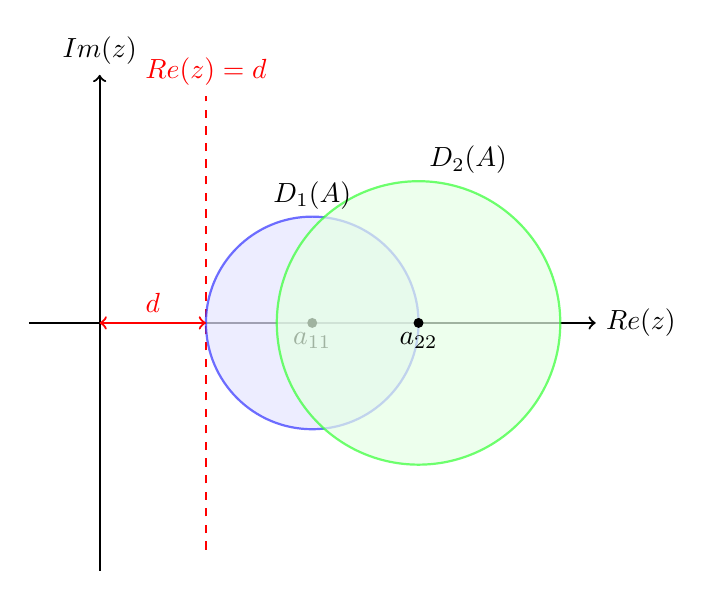
\begin{tikzpicture}[scale=0.9]
        % Axes
        \draw[->, thick] (-1,0) -- (7,0) node[right] {$\mathfrak{Re}(z)$};
        \draw[->, thick] (0,-3.5) -- (0,3.5) node[above] {$\mathfrak{Im}(z)$};
        
        % Vertical distance line
        \draw[dashed, red, thick] (1.5,-3.2) -- (1.5,3.2) node[above] {$\mathfrak{Re}(z) = d$};
        
        % Discs
        \draw[fill=blue!10, draw=blue!80, thick, opacity=0.7] (3.0,0) circle (1.5cm);
        \fill (3.0,0) circle (2pt) node[below] {$a_{11}$};
        
        \draw[fill=green!10, draw=green!80, thick, opacity=0.7] (4.5,0) circle (2.0cm);
        \fill (4.5,0) circle (2pt) node[below] {$a_{22}$};
        
        % Annotations
        \draw[<->, thick, red] (0,0) -- (1.5,0) node[midway, above] {$d$};
        \node at (3.0, 1.8) {$\mathfrak{D}_1(A)$};
        \node at (5.2, 2.3) {$\mathfrak{D}_2(A)$};
    \end{tikzpicture}
    \caption{Geometric illustration of Gershgorin discs bounded away from the origin by a minimum real separation distance $d > 0$.}
    \label{fig:gershgorin_concept}
\end{figure}

In Chapter 3, Gershgorin's Disc Theorem is applied to shift matrix sub-blocks to design local node and edge perturbation factors that enforce a minimal separation distance $d \ge 1/\gamma^2$  of the non-zero eigenvalue of the Laplacian with the smallest real part from the imaginary axis, thereby guaranteeing second-order consensus.

\subsubsection{The Ramifications of Feedback Cycles in Networks}
A foundational result in consensus theory states that a networked system can achieve state agreement over a directed graph if and only if the communication topology $\mathcal{G}$ contains a directed spanning tree (a rooted out-branching)— a subgraph where at least one node (the root or leader node) has a directed path to every other node in the network. 

In physical networks, directed cycles (or feedback loops) arise naturally due to bidirectional spatial proximity, feedback mechanisms between lower and higher organizational tiers, or reverse-edge communication channels. For example, in an autonomous vehicular platoon moving over a directed chain topology, information primarily flows downstream (vehicle $i-1$ to vehicle $i$). However, if a downstream vehicle transmits spatial coordinates back to an upstream vehicle to enforce tight inter-vehicular spacing, a closed directed cycle is formed. Directed loops present a critical dichotomy in multi-agent networks:
\begin{itemize}
    \item \textbf{The Single-Integrator Case:} For first-order networks, the introduction of reverse edges leading to directed cycles merely degrades the algebraic connectivity (Fiedler eigenvalue) and slows down the rate of convergence to consensus, without jeopardizing consensus altogether.
    \item \textbf{The Double-Integrator Case:} For second-order networks, directed cycles introduce complex-conjugate eigenvalues with imaginary components into the graph Laplacian spectrum. These complex eigenvalues induce phase lag between position alignment and velocity damping. If the velocity coupling parameter $\gamma$ falls below a critical lower bound, this phase lag can cause severe dynamic instability, leading to complete breakdown of consensus despite the presence of a directed spanning tree.
\end{itemize}

\subsection{Incidence Matrices, Edge Factorizations, and Tree Decompositions}
To enable disturbance attenuation and $\mathcal{H}_2$ norm analysis (as developed in Chapter \ref{ch:Robustness_Analysis}), we consider a network of double-integrator agents operating over an undirected path graph. For an effective $\mathcal{H}_2$ performance evaluation, the network dynamics are more conveniently expressed using edge-based state representations rather than traditional node-based coordinates. This transformation isolates and eliminates the zero eigenvalue of the graph Laplacian, thereby yielding a non-singular, reduced-order Laplacian structure required for internal stability and transfer function formulation. A non-singular structure is needed to ensure the state matrix $\mathcal{A}_x$ is Hurwitz, allowing the computation of controllability/observability Gramians and the transfer function $G(s) = \mathcal{C}_z(sI - \mathcal{A}_x)^{-1}\mathcal{B}_w$.

A comprehensive treatment of the graph-theoretic definitions and edge-space formulations presented in this section can be found in \cite{zelazo2007agreement, zelazo2009h2, zelazo2010edge}.

Let $e = |\Eg|$ denote the total number of edges in the graph $\G$. Assign an arbitrary orientation index $k \in \{1, 2, \dots, e\}$ to each edge $(j, i) \in \Eg$.

\begin{definition}[Incidence Matrix]\label{def:incidence_matrix}
The node-edge incidence matrix $E(\G) \in \R^{N \times e}$ of an undirected graph $\G$ has its $(i, k)$-th entry defined as:
\begin{equation}
    [E(\G)]_{ik} = \begin{cases}
        +1, & \text{if vertex } i \text{ is the head (destination) of directed edge } k \\
        -1, & \text{if vertex } i \text{ is the tail (source) of directed edge } k \\
        0, & \text{otherwise}
    \end{cases}
\end{equation}
For an unweighted undirected graph, the relationship between the node Laplacian $\mathcal{L}$ and the incidence matrix $E(\G)$ is given by:
\begin{equation}
    \mathcal{L} = E(\G) E(\G)^T
\end{equation}
The edge Laplacian matrix $\mathcal{L}_e \in \R^{e \times e}$ is defined dually as:
\begin{equation}
    \mathcal{L}_e = E(\G)^T E(\G)
\end{equation}
\end{definition}
\begin{definition}[Spanning Tree Factorization of the Incidence Matrix] \label{def:spanning_tree_factorization}
\leavevmode\par\noindent
Consider a graph $\G$ containing a spanning tree. By topological reordering of the edge columns, the incidence matrix $E(\G)$ can be partitioned into tree edges and cycle-closing edges:
\begin{equation}
    E(\G) = \begin{bmatrix} \etree & E_c \end{bmatrix}
\end{equation}
where $\etree \in \R^{N \times (N-1)}$ represents the $N-1$ columns belonging to a chosen spanning tree, and $E_c \in \R^{N \times (e - N + 1)}$ represents the remaining $e - N + 1$ edges that form cycles.
Since the columns of $E_c$ lie in the column space spanned by $\etree$, there exists a linear transformation matrix $T \in \R^{(N-1) \times (e - N + 1)}$ such that $E_c = \etree T$. The transformation matrix $T$ is given by:
\begin{equation}
    T = (\etree^T \etree)^{-1} \etree^T E_c
\end{equation}
Thus, the full incidence matrix can be factored compactly as:
\begin{equation}\label{eq:incidence_factored}
    E(\G) = \etree \begin{bmatrix} I_{N-1} & T \end{bmatrix} =: \etree R
\end{equation}
where $R := \begin{bmatrix} I_{N-1} & T \end{bmatrix} \in \R^{(N-1) \times e}$.

The reduced tree node Laplacian $\lntree$ and reduced tree edge Laplacian $\letree$ are defined respectively as:
\begin{equation}
    \lntree = \etree \etree^T \in \R^{N \times N}, \quad \letree = \etree^T \etree \in \R^{(N-1) \times (N-1)}
\end{equation}
\end{definition}

\subsubsection{System Performance via the $\mathcal{H}_2$ Norm}
To measure noise propagation and disturbance rejection in second-order agent networks under process noise $q(t) \in \R^N$ and measurement noise $r(t) \in \R^e$, we use the $\mathcal{H}_2$ norm metric.

Consider a stable, linear time-invariant (LTI) reduced-order system $\Sigma_e$ expressed in edge coordinates:
\begin{equation}\label{eq:h2_system_def}
    \begin{aligned}
        \dot{x}_e(t) &= \mathcal{A}_x x_e(t) + \mathcal{B}_w w(t) \\
        z(t) &= \mathcal{C}_z x_e(t)
    \end{aligned}
\end{equation}
where $w(t) = [q^T(t), r^T(t)]^T$ is a vector of uncorrelated zero-mean Gaussian white noise processes, $x_e(t)$ represents relative edge states, and $z(t)$ denotes regulated output errors.

When $\mathcal{A}_x$ is Hurwitz, the squared $\mathcal{H}_2$ norm of the system transfer function $G(s) = \mathcal{C}_z (s I - \mathcal{A}_x)^{-1} \mathcal{B}_w$ is given by \cite{dullerud2013course}:
\begin{equation}\label{eq:h2_norm_trace}
    \|\Sigma_e\|_{\mathcal{H}_2}^2 = \text{trace}(\mathcal{C}_z \mathcal{P}_{\text{ctrl}} \mathcal{C}_z^T) = \text{trace}(\mathcal{B}_w^T \mathcal{P}_{\text{obs}} \mathcal{B}_w)
\end{equation}
where $\mathcal{P}_{\text{ctrl}}$ and $\mathcal{P}_{\text{obs}}$ are the controllability and observability Gramians, satisfying the Lyapunov equations:
\begin{equation}\label{eq:lyapunov_equations}
    \mathcal{A}_x \mathcal{P}_{\text{ctrl}} + \mathcal{P}_{\text{ctrl}} \mathcal{A}_x^T + \mathcal{B}_w \mathcal{B}_w^T = 0_{2(N-1), 2(N-1)}
\end{equation}
\begin{equation}
    \mathcal{A}_x^T \mathcal{P}_{\text{obs}} + \mathcal{P}_{\text{obs}} \mathcal{A}_x + \mathcal{C}_z^T \mathcal{C}_z = 0_{2(N-1), 2(N-1)}
\end{equation}

In Chapter 4, closed-form solutions for $\|\Sigma_e\|_{\mathcal{H}_2}^2$ are derived to establish how graph cycle length, spatial loop placement relative to the root node, and dual-loop overlap govern stochastic noise attenuation.


\subsection{Real-World Applications: Cooperative Guidance and Interception}
The theoretical analysis and synthesis of consensus protocols is directly connected to physical motion control in defense and aerospace engineering, specifically in coordinated interception and cooperative multi-agent guidance. In modern precision strike missions against stationary or low-maneuverability targets (such as naval vessels or ground installations), a single interceptor can be countered by Close-In Weapon Systems (CIWS).

To overcome such defensive countermeasures, swarms of autonomous interceptors need to execute coordinated attacks. This requires solving two physical constraints simultaneously:
\begin{itemize}
    \item Temporal Constraint (Impact Time $t_{\text{imp}}$): All interceptors in the swarm must intercept the target at the exact same time instant to overwhelm automated defenses.
    \item Directional Constraint (Impact Angle $\zeta$): Each interceptor must intercept the target along a designated approach angle to maximize warhead penetration or exploit blind spots of the target's radar system.
\end{itemize}
Executing these cooperative engagements under strict non-holonomic kinematics and actuator limits ($\vert{}a_M\vert{} \le a^{\text{max}}$) requires bridging the ideas of consensus theory with physical trajectory generation for individual interceptors.
\section{Problem Statements and Research Challenges}
\subsection{Consensus Breakdown and Velocity Coupling Bounds in Double-Integrator Networks}

Building upon early work on single-integrators over undirected topologies, Ren and Atkins \cite{ren2005second} extended consensus protocols to double-integrator agent dynamics over directed network topologies. Consider $N$ double-integrator agents operating under the distributed control law:
\begin{equation} \label{eq:agent-wise}
	u_i(t) = -\sum_{j=1}^{N} w_{ij} \left[ (p_i(t) - p_j(t)) + \gamma (v_i(t) - v_j(t)) \right], \quad i \in \{1, 2, \dots, N\}
\end{equation}
where $p_i(t), v_i(t) \in \mathbb{R}^d$ represent the position and velocity vectors of agent $i$, $w_{ij}$ is the $(i,j)$-th entry of the weighted adjacency matrix $\mathcal{W}$, and $\gamma > 0$ is the \textbf{velocity coupling parameter}.

In \cite{ren2005second}, it was observed that while protocol \eqref{eq:agent-wise} seamlessly achieves consensus over acyclic topologies, consensus can suddenly break down when directed cycles are present in the network graph. To guarantee consensus over general digraphs containing a directed spanning tree, Ren and Atkins established a conservative sufficient lower bound on the velocity coupling parameter $\gamma$:
\begin{equation}\label{eq:ren_gamma_bound}
    \gamma > \max_{i \in \{2, \dots, N\}} \sqrt{\frac{2}{\mathfrak{Re}(\lambda_i)}}
\end{equation}
where $\lambda_i$ denotes the $i$-th non-zero eigenvalue of the graph Laplacian matrix $\mathcal{L}$, ordered by real parts such that $0 = \lambda_1 < \mathfrak{Re}(\lambda_2) \le \dots \le \mathfrak{Re}(\lambda_N)$.

\begin{figure}[ht!]
    \centering
    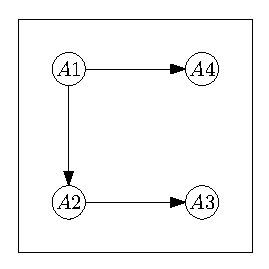
\includegraphics[width=0.6\textwidth, keepaspectratio]{Sapnning.eps}
    \caption{Consensus achieved for $\gamma = 0.1$ over an acyclic directed spanning tree topology.}
    \label{fig:spanning_tree_consensus}
\end{figure}

\begin{figure}[ht!]
    \centering
    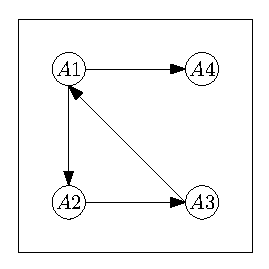
\includegraphics[width=0.6\textwidth, keepaspectratio]{Cycle.eps}
    \caption{Breakdown of consensus due to the presence of directed cycles.}
    \label{fig:cycle_consensus_failure}
\end{figure}

Subsequently, Yu et al. \cite{yu2009second, yu2010some} derived the exact necessary and sufficient condition for second-order consensus over directed topologies. Specifically, the velocity coupling factor $\gamma$ must satisfy:
\begin{equation}\label{eq:yu_gamma_exact_bound}
    \gamma > \max_{i \in \{2, \dots, N\}} \frac{|\mathfrak{Im}(\lambda_i)|}{|\lambda_i|} \sqrt{\frac{1}{\mathfrak{Re}(\lambda_i)}}
\end{equation}
where $|\lambda_i| = \sqrt{\mathfrak{Re}(\lambda_i)^2 + \mathfrak{Im}(\lambda_i)^2}$ is the magnitude of the $i$-th Laplacian eigenvalue.

In acyclic networks (such as directed chains or trees), all non-zero Laplacian eigenvalues are purely real ($\mathfrak{Im}(\lambda_i) = 0$), reducing the right-hand side of \eqref{eq:yu_gamma_exact_bound} to zero and permitting consensus for any arbitrarily small choice of $\gamma > 0$. However, when directed cycles exist, complex-conjugate eigenvalue pairs emerge with non-zero imaginary parts ($\mathfrak{Im}(\lambda_i) \neq 0$), imposing a strictly positive lower bound on $\gamma$. 

If an operational network has a fixed, predesigned velocity coupling factor $\gamma$, the introduction of reverse feedback channels shifts the Laplacian spectrum outward in the complex plane, potentially violating condition \eqref{eq:yu_gamma_exact_bound} and triggering system instability.

This vulnerability under cyclic topologies motivates the core research problem addressed in the chapter \ref{ch:TwoReverseEdges}:
\begin{problem}\label{prob:multi_loop_coupling}
    Analyze how the presence of multiple interacting directed loops (whether disjoint, overlapping, or sharing root/leader nodes) modifies the analytical bounds on the velocity coupling parameter $\gamma$ across chain topologies, and formulate local edge/node perturbation methodologies to guarantee consensus under fixed coupling constraints.
\end{problem}
\subsection{The Root-Node Loop Structural Singularity}
Standard polynomial-based spectral analysis techniques (such as Routh-Hurwitz criteria on Laplacian characteristic equations) rely on the root node (leader) having an in-degree of zero ($d_{in,1} = 0$). Under this condition, the root node acts as an autonomous leader unaffected by downstream feedback.

However, when a reverse communication edge enters the root node itself ($x_1 = 1$), such a hierarchical structure, which preserves the root node, collapses. The root node loses its hierarchical immunity ($d_{in,1} > 0$), and \textbf{every node within the directed cycle effectively becomes an equivalent root node}.
\begin{problem}
    When the leader/root participates in a loop, standard characteristic polynomials yield trivial solutions ($s_1 = 1$), failing to provide reliable stability bounds. The literature lacks a fully decentralized framework capable of guaranteeing consensus when the root node is embedded in a loop, without requiring agents to access global spectrum knowledge or retune the global parameter $\gamma$. Address this issue by possibly designing a local gain-tuning strategy in the face of such a loop-formation.
\end{problem}
\subsection{$\mathcal{H}_2$ Performance and Disturbance Attenuation in Cyclic Topologies}
Beyond deterministic convergence, real-world multi-agent networks operate under environmental disturbances and sensor noise. The $\mathcal{H}_2$ norm measures total transient energy and stochastic noise amplification from exogenous inputs to network state deviations.

In single-integrator networks, it is known that the $\mathcal{H}_2$ performance is invariant to the choice of spanning tree and cycle location. For double-integrator networks, however, state dynamics are coupled through position and velocity integrators and such relationships or lack thereof between the performance and the choice of some specific spanning trees is largely unexplored.

\begin{problem}
    Derive, if possible, closed-form expressions for the $\mathcal{H}_2$ norm in a network of consensus-seeking double-integrators over path graphs. Quantify how cycle length, spatial placement of cycles relative to the root node, and partial structural overlap between two cycles dictate the overall $\mathcal{H}_2$ performance. 
\end{problem}
\subsection{Trajectory Planning under Non-Holonomic and Spatio\-temporal Constraints}
Translating consensus principles to physical autonomous interceptors introduces kinematic and dynamic constraints. Classical Proportional Navigation Guidance (PNG) and Dubins curves suffer from major physical limitations:
\begin{itemize}
    \item Dubins Rigidity: Standard Dubins paths use fixed minimum turn radii ($r_m$), that do not offer any flexibility in the choice of \emph{impact time} or an interception mission's duration.
    \item Acceleration Bounds: Physical actuators saturate at $a^{\text{max}}$. If initial engagement geometry is unfavorable, standard guidance laws demand unachievable lateral acceleration ($a_M > a^{\text{max}}$), causing the interceptor to miss its target. 
\end{itemize}
\begin{problem}
    Develop continuous-curvature, and acceleration-bounded guidance strategies that guarantee simultaneous satisfaction of spatial impact angle ($\zeta$) and temporal impact time ($t_{\text{imp}}$) constraints for single interceptors, and then extend such ideas to multi-interceptor teams by possibly exploiting the idea of consensus.
\end{problem}
\section{Literature Review and State-of-the-Art}
The theoretical foundations of this dissertation leads to intersection of several key domains in control theory, algebraic graph theory, and autonomous motion planning such as: consensus protocols for second-order multi-agent systems, spectral analysis of cyclic directed graphs, network performance optimization under stochastic disturbance, and constrained spatial-temporal trajectory synthesis. This section provides a crucial, structured review of the state-of-the-art across these interconnected domains, while explicitly identifying the theoretical gaps that motivate our contributions.

\subsection{Consensus Protocols for High-Order Multi-Agent Systems}
The systematic study of consensus protocols— where a group of autonomous agents achieves agreement on a common state vector via localized interaction— began with foundational works on first-order (single-integrator) systems \cite{saber2003consensus, jadbabaie2003coordination, fax2004information, 1333204}. Olfati-Saber and Murray \cite{saber2003consensus} established the basic graph-theoretic framework for consensus over fixed and switching topologies, proving that convergence depends on the algebraic connectivity (the Fiedler value, $\lambda_2$) of the graph Laplacian. Moreau \cite{moreau2005stability} extended these results to time-dependent directed communication links using set-valued Lyapunov functions.

However, physical robotic platforms, UAVs, and mechanical actuators are governed by double-integrator dynamics where acceleration or force acts as the control input. Ren and Beard \cite{ren2005second} introduced second-order consensus protocols, demonstrating a fundamental difference between first- and second-order systems: while a directed spanning tree is necessary and sufficient for first-order consensus, it is only \emph{ necessary} for second-order consensus. Over a directed graph, double-integrator consensus can fail even in the presence of a directed spanning tree, due to the phase lag introduced by complex Laplacian eigenvalues.

Ren \cite{ren2008consensus} subsequently derived a sufficient condition for second-order consensus based on the real parts of the Laplacian spectrum, establishing that a positive velocity coupling gain $\gamma$ must be selected above a critical threshold. This formulation was further refined to handle practical constraints such as actuator saturation and velocity measurement unavailability \cite{ren2008consensus}. A major breakthrough was achieved by Yu et al. \cite{yu2010some}, who derived the exact \textbf{necessary and sufficient condition} for second-order consensus over directed graphs. Their analytical criterion proved that convergence depends on both the real and imaginary components of the Laplacian spectrum:
\begin{equation}\label{eq:ch1_nec_suf}
    \gamma > \max_{i \in \{2, \dots, N\}} \frac{|\mathfrak{Im}(\lambda_i)|}{|\lambda_i|} \sqrt{\frac{1}{\mathfrak{Re}(\lambda_i)}}
\end{equation}
Despite these analytical advancements, existing double-integrator control laws assume global knowledge, such as that of the Laplacian spectrum, available with every agent. When structural changes occur in a network, existing approaches require every agent in the network to access information about the graph eigenvalues and re-tune their velocity coupling parameter $\gamma$ globally. Existing results in the literature lack decentralized, localized tuning/re-tuning methods that allow agents on modified edges to restore stability locally without requiring global network re-tuning.

\subsection{Cyclic Directed Networks and Spectral Instability}
Feedback loops and directed cycles occur naturally in networked physical systems due to bidirectional links, spatial proximity, and multi-tiered communication architectures. In single-integrator networks, the inclusion of reverse edges creating directed loops merely degrades the convergence rate to consensus by reducing algebraic connectivity, but never induces dynamic instability. 

The spectral properties of weighted digraphs and cyclic graphs have been investigated from various perspectives \cite{mukherjee2016consensus, mukherjee2013reachability, mukherjee2021finite}. Zhang et al. \cite{zhang2017effect} analyzed the effect of adding a reverse edge across a stem in a directed acyclic graph (DAG) for single integrators, concluding that convergence degradation is dictated exclusively by the subgraph encompassing the directed cycle and remains invariant to total network size or cycle location. Mo et al. \cite{mo2019effects} expanded this analysis to consider reverse edges across stems in DAGs.

For chain networks containing dual reverse edges, Hao et al. \cite{hao2019role} evaluated the dominant convergence root of single-integrator consensus, establishing polynomial equations to estimate eigenvalue shifts. However, the analytical framework in \cite{hao2019role} suffers from two major limitations:
\begin{itemize}
    \item \textbf{Topological Restrictions:} Their derivations are valid only when the lengths of the two cycles, induced by the addition of two reverse-edges, differ by at least 1 ($|l_1 - l_2| \ge 1$) and when the longer cycle is located strictly closer to the root node.
    \item \textbf{Root-Node Loop Failure:} When a reverse edge enters the root node itself ($x_1 = 1$), the polynomial spectral methods fail to yield any conclusive answers. Because the root node loses its zero in-degree property ($d_{\text{in},1} > 0$), every node within the cycle effectively transforms into an equivalent root node. In such a set-up, the relevant characteristic equations of interest yield trivial solutions ($s_1 = 1$), thereby rendering the proposed polynomial methods unable to provide any bounds on the velocity coupling factor.
\end{itemize}

Resolving consensus breakdown when the leader/root node is embedded in a feedback loop— a structural singularity that destroys traditional leader-follower hierarchies— remains an unaddressed problem in the literature.

\subsection{$\mathcal{H}_2$ Performance and Disturbance Attenuation in Networked Systems}
Beyond deterministic convergence, real-world multi-agent networks operate under process noise and measurement disturbances. To quantify stochastic noise amplification, researchers employ system norm performance metrics, specifically the $\mathcal{H}_2$ and $\mathcal{H}_\infty$ norms.

Zelazo and Mesbahi \cite{zelazo2010edge} developed an edge-agreement framework using the edge Laplacian ($\mathcal{L}_e = E^T E$), enabling reduced-order realization of network dynamics by eliminating the zero Laplacian eigenvalue. Zelazo et al. \cite{zelazo2013performance} utilized this framework to analyze the $\mathcal{H}_2$ performance of single-integrator networks over cyclic graphs. Their fundamental conclusion was that for first-order agents, $\mathcal{H}_2$ performance depends strictly on cycle length and is completely invariant to the choice of spanning tree or the spatial location of the cycle in the graph.

The performance of second-order networks under update delays and spectral variations has been studied by Huang and Siami \cite{huang2022role} and Oral et al. \cite{oral2017performance}. However, the $\mathcal{H}_2$ performance of double-integrator networks over cyclic topologies remains under-explored. Unlike single-integrators, second-order agents possess coupled position and velocity dynamics. Consequently, fundamental questions regarding how cycle length, spatial loop placement relative to the root node, and partial structural overlap between dual loops affect $\mathcal{H}_2$ performance in second-order networks remain open questions.

\subsection{Impact-Angle and Impact-Time Constrained Guidance Laws}
Translating graph theory-aided consensus protocols to physical robotic platforms and autonomous UAVs/interceptors requires trajectory planning under non-holonomic constraints, limited speed, and saturated lateral acceleration ($|a_M| \le a^{\text{max}}$).

In defense and aerospace applications, cooperative engagements require satisfying two terminal constraints simultaneously: exact impact time ($t_{\text{imp}}$) to saturate close-in weapon systems (CIWS), and exact impact angle ($\zeta$) to maximize directional warhead penetration. 

Classical Proportional Navigation Guidance (PNG) \cite{SHNEYDOR1998101} and Pure Pursuit (PP) \cite{SHNEYDOR199847} guarantee interception but cannot enforce terminal impact angles without demanding excessive terminal acceleration. Biased PNG laws \cite{kim1998BPNG} and optimal impact-angle guidance laws \cite{Ryoo, ratnoo2009state} attempt to enforce directional constraints but often exhibit command singularities or require time-to-go polynomial approximations.

To satisfy simultaneous impact-angle and impact-time constraints, several strategies have been proposed:
\begin{itemize}
    \item Sliding Mode and Lyapunov Methods: Kumar et al. \cite{kumar2012sliding}, Tekin et al. \cite{Tekin2016_IT}, and Chen \& Wang \cite{Chen2018JGCD} developed sliding-mode and Lyapunov-based guidance laws for time and angle control. While robust, these methods typically produce high-frequency chatter or severe acceleration spikes near terminal intercept.
    \item Augmented Bias and Backstepping: Zhang et al. \cite{zhang2013terminal, Zhang2015} and Jung \& Kim \cite{Jung2006} formulated impact time and angle guidance laws using linear frame assumptions. However, these methods deteriorate under large initial heading errors ($\theta_M \approx 90^\circ$).
    \item Geometric Trajectory Shaping: Hota and Ghose \cite{hota2009modified} utilized Dubins paths for UAV convergent line tracking. However, standard Dubins paths use fixed minimum turn radii ($r_m$), resulting in rather inflexible values of impact time when implemented.
    \item Spiral Trajectory Synthesis: Tripathy and Shima \cite{tripathy2019archimedean} and Mishra et al. \cite{mishra2024spiral} introduced Archimedean spiral guidance laws for impact-angle control. Spirals inherently encode the desired impact angle while providing smooth curvature decay. However, existing spiral guidance laws do not guarantee feasibility under strict actuator limits ($|a_M| \le a^{\text{max}}$); if initial engagement geometry is unfavorable, standard spiral laws demand unachievable lateral acceleration, leading to target miss.
\end{itemize}



\subsection{Summary of Identified Gaps in the Literature}
Table \ref{tab:literature_gaps} summarizes the state-of-the-art gaps identified across the four aforesaid domains, and contrasts them with the specific contributions developed in this dissertation.

\begin{table}[ht!]
\centering
\caption{Comparison between state-of-the-art limitations and thesis contributions.}
\label{tab:literature_gaps}
\renewcommand{\arraystretch}{1.3}
\begin{tabularx}{\textwidth}{|>{\raggedright\arraybackslash}p{3cm}|>{\raggedright\arraybackslash}X|>{\raggedright\arraybackslash}X|>{\raggedright\arraybackslash}X|}
\hline
\textbf{Research Domain} & \textbf{State-of-the-Art Approaches} & \textbf{Identified Gap / Limitation} & \textbf{Thesis Contribution} \\ \hline

\textbf{Second-Order Directed Consensus} & Ren \& Beard \cite{ren2008consensus}, Yu et al. \cite{yu2010some}, Zhang et al. \cite{zhang2017effect}, Hao et al. \cite{hao2019role}. & Global spectrum knowledge required to re-tune $\gamma$; polynomial methods fail when root/leader is inside a loop. & Characterized dual-loop interaction bounds; developed local node/edge scaling and root-locus remedies for root-node loops. \\ \hline

\textbf{Network $\mathcal{H}_2$ Performance} & Zelazo et al. \cite{zelazo2013performance}, Huang \& Siami \cite{huang2022role}, Oral et al. \cite{oral2017performance}. & $\mathcal{H}_2$ norm of double integrators over cyclic graphs not analyzed; impact of spatial loop placement and overlap unknown. & Derived closed-form $\mathcal{H}_2$ norm for double integrators on path graphs; proved spatial centering and partial overlap optimize noise rejection. \\ \hline

\textbf{Space-Time Guidance Laws} & Harl \& Balakrishnan \cite{harl2011impact}, Zhang et al. \cite{Zhang2013}, Tekin et al. \cite{Tekin2016_IT}. & Discontinuous curvature ($\dot{\kappa} = \infty$), command singularities at large heading errors, time-to-go estimation errors. & Formulated piecewise-constant acceleration Dubins guidance; introduced feasibility-seeking Archimedean spiral guidance with continuous curvature. \\ \hline

\textbf{Cooperative Coordination} & Zhao et al. \cite{zhao2015terminal}, Park et al. \cite{park2013optimal}, Chen \& Wang \cite{Chen2018AST}. & Centralized synchronization assumptions; unconstrained actuator saturation; limited spatial sector flexibility. & Integrated Archimedean spiral guidance with directed chain consensus, guaranteeing both impact along chosen spatial sectors and adherence to acceleration bounds. \\ \hline
\end{tabularx}
\end{table}
\section{Research Objectives and Scope}
The overarching objective of this dissertation is to establish a unified framework spanning algebraic graph-theoretic stability analysis, performance optimization, and physical trajectory synthesis for constrained multi-agent systems. The specific research objectives are:
\begin{itemize}
    \item \textbf{Objective 1 (Loop Bound Characterization):} Derive exact analytical characteristic equations and velocity coupling bounds for double-integrator multi-agent systems operating over directed chain topologies with two interacting reverse edges across all topological overlap configurations.
    \item \textbf{Objective 2 (Decentralized Local Consensus Restoration):} Formulate local node-scaling, edge-scaling, and combined perturbation algorithms that guarantee second-order consensus for a fixed $\gamma$ without global spectrum access. Develop a root-locus design framework to resolve the root-node loop singularity.
    \item \textbf{Objective 3 ($\mathcal{H}_2$ Performance Guidelines):} Derive closed-form expressions for the $\mathcal{H}_2$ norm of second-order agent networks on path graphs. Characterize optimal cycle length, spatial positioning relative to the root node, and structural overlap for dual loops to minimize noise amplification. 
    \item \textbf{Objective 4 (Space-Time Dubins Trajectory Synthesis):} Design a Dubins-type guidance law using piecewise-constant lateral acceleration profiles to satisfy simultaneous impact angle and impact time constraints under strict lateral acceleration limits.
    \item \textbf{Objective 5 (Continuous-Curvature Spiral Guidance \& Swarm Coordination):} Develop an (possibly two-phase) adaptive Archimedean spiral guidance strategy that enforces curvature feasibility under actuator saturation ($a^{\text{max}}$). Unify spiral trajectory generation with consensus protocols over digraphs for coordinated interception.
\end{itemize}

\section{Thesis Contributions and Novelty}
The primary analytical and application-oriented contributions of this thesis are summarized as follows:
\begin{itemize}
    \item \textbf{Dual-Loop Spectral Characterization in Directed Chains:} We establish exact univariate polynomial equations that dictate the dominant Laplacian convergence root $s_1 = 1 - \lambda_2$ across six distinct topological configurations of dual reverse edges. We prove that adding a cycle of length $l$ alters $l+1$ eigenvalues when the root node is excluded, but only $l$ eigenvalues when the root node is included.
    \item \textbf{Local Decentralized Perturbation Framework (Leader-Exterior Loops):} We introduce Gershgorin-disc-based Node Scaling, Edge Scaling, and Combined Scaling methods. By constructing Arithmetic Progressions (AP) of disc centers, these strategies guarantee second-order consensus for any predesigned coupling gain $\gamma$ through localized modifications confined strictly to loop edges and nodes.
    \item \textbf{Resolution of the Root-Node Loop Structural Singularity:} We provide the first framework in the literature to resolve consensus breakdown when the leader node is inside a feedback loop. Using a complementary root-locus formulation wherein a relevant transfer function of the form $G(s) = \frac{\beta_{RL}\{(s-\alpha_{RL})^l - (-\alpha_{RL})^l\}}{s(s-\alpha_{RL})^l}$ is used, we derive precise gain bounds that preserve stability. Furthermore, we prove that an equal-weight cyclic pursuit design ($\alpha_{RL} \ge \frac{\cot^2(\pi/(l+1))}{2\gamma^2}$) guarantees consensus without requiring edge weakening.
    \item \textbf{Closed-Form $\mathcal{H}_2$ Performance Expressions and Structural Guidelines:} We derive exact closed-form expressions for the $\mathcal{H}_2$ norm of double-integrator networks over path graphs. We prove that: 
        \begin{itemize}
            \item Double integrators inherently exhibit higher noise sensitivity than single integrators, but increasing velocity coupling ($\gamma$) monotonically improves $\mathcal{H}_2$ performance.
            \item Placing a single cycle at the spatial center of a path graph ($n_c = \frac{n+1}{2}$) minimizes the effects of noise.
            \item For two loops/cycles, partial overlap between cycles ($s > 0$) strictly improves $\mathcal{H}_2$ performance, compared to non-overlapping loop configurations.
        \end{itemize}
    \item \textbf{Dubins Type Path Based Space-Time Guidance Scheme:} We design a piecewise-constant acceleration guidance law that modulates a virtual design circle radius $r_d \in [r_m, r_{\text{crit}}^{\text{TCT}}]$ to hit simultaneous terminal impact angle and impact time constraints. We eliminate upper impact-time bounds by introducing a mirrored launch configuration. 
    \item \textbf{Feasibility-Seeking Archimedean Spiral Guidance and Cooperative Control:} We formulate a two-phase guidance strategy that dynamically adapts the spiral parameter $\alpha$ via $\dot{\alpha} = K_p(\alpha_{\text{ref}} - \alpha)$ to guarantee curvature feasibility under actuator saturation ($a^{\text{max}}$). By coupling spiral parameter generation with directed graph consensus ($\alpha_i \to \alpha_{\text{ref}}$), we achieve coordinated multi-agent interception across prescribed spatial impact sectors.
\end{itemize}

\section{Thesis Organization and Outline}\label{sec:thesis_organization}

This dissertation is organized into the following chapters, structured to systematically bridge consensus based on algebraic graph theory, and performance optimization based on system theory, with physical trajectory synthesis for constrained autonomous systems:

\begin{itemize}
    \item \textbf{Chapter \ref{ch:intro}: Mathematical Preliminaries and Fundamental Concepts} \\
    This chapter establishes the foundational mathematical framework used throughout the dissertation. This includes algebraic graph theory (adjacency, in-degree, and Laplacian matrices, topological ordering, incidence matrix factorizations, and reduced edge Laplacians), dynamical agent models (second-order/double-integrator dynamics, Kronecker state-space formulations, and classical stability criteria), planar non-holonomic engagement kinematics, and geometric curve primitives (Dubins circles and Archimedean spirals).
    
    \item \textbf{Chapter \ref{ch:TwoReverseEdges}: Consensus Analysis of Dual Loops in Directed Networks } \\
    Next, this chapter investigates the spectral impact of reverse edges added across directed chain networks of double integrators. Exact characteristic polynomial equations and dominant convergence roots are derived across six topological configurations of two reverse edges. The structural singularity that occurs when the root/leader node is embedded within a directed cycle is formally characterized.
    \item \textbf{Chapter \ref{ch:Guaranteed_Consensus}: Guaranteed Consensus via Edge-Weight Perturbation in Directed Loop Topologies}
    This chapter presents detailed derivations for dual-loop spectral bounds, characterizes the root-node loop structural singularity, and details decentralized node-scaling, edge-scaling, combined scaling, and root-locus based remedies. To resolve consensus breakdown without global spectrum re-computation, localized node-scaling, edge-scaling, combined scaling, and root-locus based remedies are proposed.
    \item \textbf{Chapter \ref{ch:Robustness_Analysis}: $\mathcal{H}_2$ Performance Analysis of Cyclic Network Topologies} \\
    This chapter evaluates systematic disturbance rejection and stochastic noise amplification in networks of consensus-seeking double integrators, specifically over directed path graphs, under process and measurement noise. Utilizing reduced-order edge dynamics ($\Sigma_{e\tau}$), exact closed-form Lyapunov solutions relevant for evaluating the $\mathcal{H}_2$ norm are derived. Quantitative structural guidelines are established, proving that spatial loop centering and partial overlap between two loops aid in optimizing the $\mathcal{H}_2$ performance.
    
    \item \textbf{Chapter \ref{ch:Dubins_Path}: Trajectory Planning Using Dubins-like Paths Under Impact Constraints} \\
    In this chapter, we present a space-time trajectory generation strategy for autonomous interceptors, subject to non-holonomic constraints, lateral acceleration bounds ($|a_M| \le a^{\text{max}}$), and simultaneous terminal impact-angle ($\theta_t$) and impact-time ($t_{\text{imp}}$) constraints. Modulating a virtual design circle radius ($r_d$) generates piecewise-constant acceleration profiles with closed-loop realizability, while a mirrored launch geometry eliminates upper bounds on achievable impact-time values.
    
    \item \textbf{Chapter \ref{ch:Spiral_Path}: Archimedean Spiral Guidance and Cooperative Multi-Agent Interception} \\
    This chapter formulates a continuous-curvature, two-phase Archimedean spiral guidance law that dynamically adapts a spiral parameter, $\alpha$, to guarantee feasibility prior to terminal tracking, while preventing actuator saturation. This synthesis is subsequently extended to a group of multi-interceptors by coupling spiral trajectory generation with a directed consensus in spiral scaling parameters ($\alpha_i \to \alpha_{\text{ref}}$), achieving coordinated interception across prescribed spatial sectors.
    
    \item \textbf{Chapter \ref{ch:conclusion}: Conclusions and Future Research Directions} \\
    Finally, this chapter summarizes the key theoretical contributions, algebraic graph-theoretic insights, and motion control methodologies developed in this dissertation, and highlights practical deployment considerations for vehicular swarms, while laying out promising avenues for future research.
\end{itemize}
